\documentclass[12pt]{beamer}

% \usepackage{cmap}
\usepackage[english, russian]{babel}

\usetheme{metropolis}
\usepackage{appendixnumberbeamer}

\usepackage{booktabs}
\usepackage{minted}
\usepackage[many]{tcolorbox}
\usepackage{mdframed}

\usepackage{listings}
\lstset{basicstyle=\ttfamily\small,
	showstringspaces=false,
	breaklines=true,
	frame=lrtb,
	% numbers=left,
	extendedchars=\true,
	language=Java
}

\usepackage{xcolor}

\usepackage{xspace}
\newcommand{\themename}{\textbf{\textsc{metropolis}}\xspace}

\title{Автоматизация миграции программного кода на новый набор библиотек}
\author[Алексюк Артем]{
    Студент: Алексюк Артем\\
    гр. 63501/3\\ \\
    Руководитель: Ицыксон В.М.\\
    Аттестация №2
}
\date{\today}

\begin{document}

\maketitle

\begin{frame}
\frametitle{Разработка инструментального средства}

\begin{itemize}
    \item Цели
        \begin{itemize}
            \item ...
        \end{itemize}
    \item Требования
        \begin{itemize}
            \item Поддержка миграции кода на языке Java
            \item Извлечение различных моделей анализируемой системы
            \item Встроенные средства отображения
            \item Модульная расширяемая структура
            \item Экспорт разных артефактов системы во внешние отчеты
            \item Предоставление API к разработанным методам анализа
        \end{itemize}
\end{itemize}
\end{frame}

\begin{frame}[fragile]{Пример задачи миграции}
	Программа, использующая библиотеку java.net.URLConnection:
\begin{minted}[breaklines,fontsize=\small]{java}
URL url = new URL("http://api.ipify.org/");
URLConnection conn = url.openConnection();
\end{minted}
	Программа, использующая библиотеку Apache HttpClient:
\begin{minted}[breaklines,fontsize=\small]{java}
CloseableHttpClient httpclient = HttpClients.createDefault();
HttpGet httpget = new HttpGet("http://api.ipify.org/");
CloseableHttpResponse httpResponse = httpclient.execute(httpget);
\end{minted}
\end{frame}

\begin{frame}{Общая схема решения задачи}
	\begin{center}
		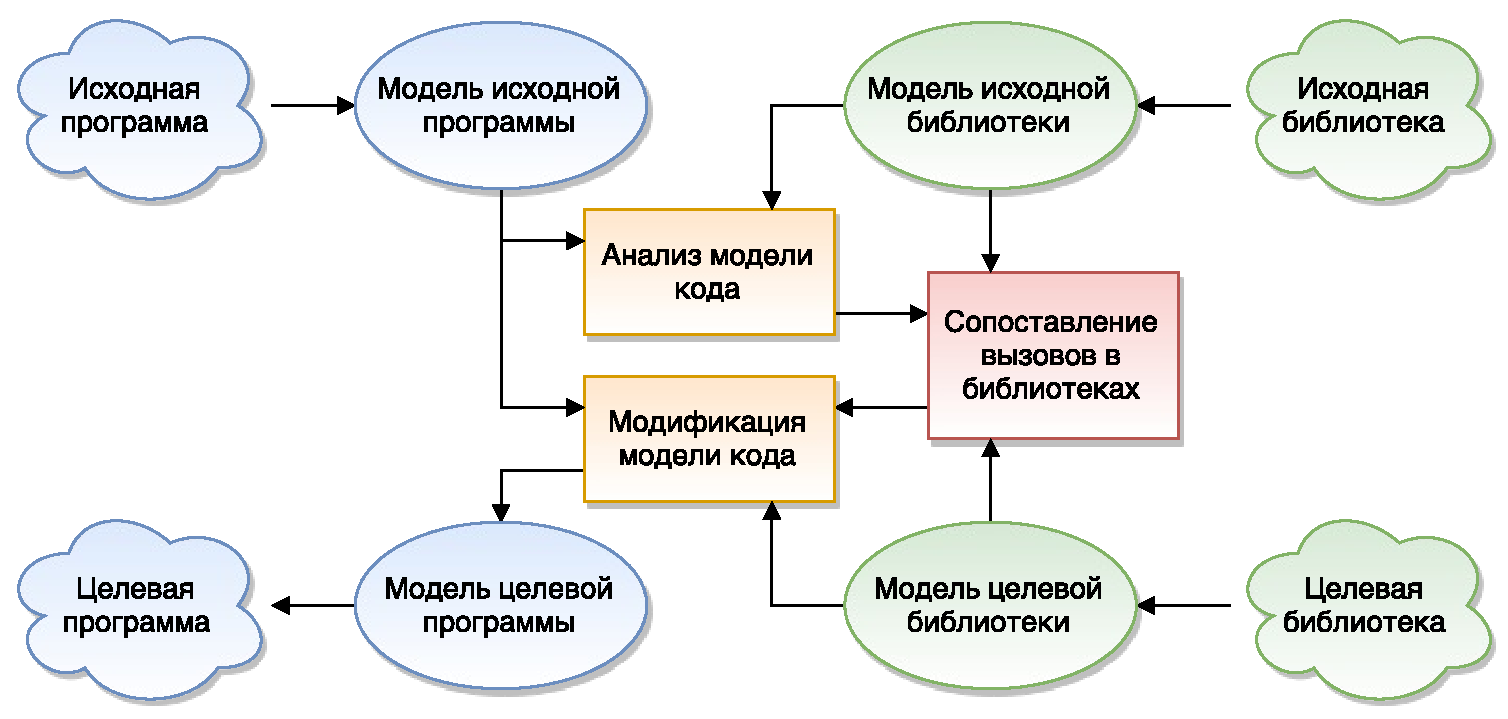
\includegraphics[width=\textwidth]{scheme.pdf}
	\end{center}
\end{frame}

\begin{frame}
\frametitle{Разработка}

\begin{itemize}
    \item Разработка метамодели
        \begin{itemize}
            \item Стандарт MOF (Meta Object Facility)
        \end{itemize}
    \item Выбор промежуточного представления
        \begin{itemize}
            \item XMI (XML Metadata Interchange)
        \end{itemize}
    \item Разработка преобразователей
        \begin{figure}[h!]
            \begin{center}
                \includegraphics[width=0.9\textwidth]{img/parser_architecture.png}
            \end{center}
        \end{figure}
\end{itemize}

\end{frame}

\begin{frame}
\frametitle{Направления дальнейшей разработки}

\begin{itemize}
    \item Реализация преобразователя для языка Java
    \item Разработка методов трансформации и алгоритмов над метамоделью
    \item Разработка графического интерфейса
    \item Разработка библиотеки моделей
\end{itemize}
\end{frame}

\begin{frame}{План работы}
    \begin{itemize}
        \item[\checkmark] формулировка требований к среде
        \item[\checkmark] анализ существующих решений
        \item[\checkmark] постановка задачи магистерского исследования
        \item[\checkmark] анализ требований к среде
        \item[\checkmark] проектирование архитектуры среды
        \item проектирование API среды
        \item реализация
        \item тестирование
        \item написание пояснительной записки
    \end{itemize}
\end{frame}

\begin{frame}[t]{Контакты}
	Email: artyom.h31@gmail.com
	
	GitHub: \url{https://github.com/h31/LibraryMigration}
	
	\vspace{1cm}
	\begin{center}
		\Large
		Спасибо за внимание!
	\end{center}
\end{frame}

\end{document}
